\section{Detailed experimental methods}
\label{app:methods}
This appendix specifies the completed core, feature-response, and readout-repair experiments. It reports the settings used in those fits and estimates from the development population.

\subsection{Movement generation, observations, and normalization}
Preparation selects walking candidates by motion name from eligible AMASS motions, divides them into nonoverlapping 128-frame windows, and screens projected geometry. These selection criteria do not verify clinical status or natural gait in every interval. The edit composes a local right-knee rotation with recorded body-model motion. An ankle-height proxy gates the rotation, which tapers to zero at window boundaries. Edit levels are 0, 5, 10, and 15 degrees. Editing comes before reflection about a pelvis-defined plane and exchange of body-model side indices. Cameras are fitted once across each window's original, edited, and mirrored geometries, then kept fixed. Oblique and side views use 45 and 90 degrees. The nominal rotation need not equal the resulting 2D angle change.

Rendered person boxes are supplied to the fixed estimators. The selected joints, in bilateral pairs, are shoulders, elbows, wrists, hips, knees, and ankles. Naming corruption permutes the coordinate, confidence, and availability channels together; timestamps and anatomically labeled references are unchanged. Global swaps affect the full sequence; temporary swaps cover its middle third. Image occlusion and artificial pretraining masks are different operations. Reference coordinates are projected body-model joints, including joints hidden in an image. They are exact for this chosen model and projection, not independently measured anatomy.

For endpoint $i$, let $O_i(t,j)$ be observation availability and $M_i(t,j)$ the artificial query mask repeated over four-frame patches. Context is $C_i=O_i\wedge\neg M_i$. Normalization uses only context coordinates:
\begin{equation}
o_i=\operatorname{median}(X_{C_i}),\qquad
s_i=\|P_{95}(X_{C_i})-P_5(X_{C_i})\|_2,\qquad
\widetilde X_i=(X_i-o_i)/s_i.
\end{equation}
Medians and percentiles operate separately on the two axes. With fewer than two context points, a nonfinite span, or span below $10^{-6}$, the recorded fallback is $o_i=(0,0),s_i=1$. References and hidden input coordinates cannot affect this transform. Teacher references use the same endpoint-specific observation transform; predictions return to pixels by $\widehat Y_i=s_i\widehat Y_i^{\rm norm}+o_i$. Inference adds no artificial mask.

\subsection{Tokens, masking, and readout}
Each four-frame joint patch contains five channels per frame: coordinates with unavailable values zeroed, confidence, availability, and seconds since the first timestamp. A linear $20\to96$ map, learned joint embedding, and sinusoidal time position form 384 tokens. The encoder has four layers and four attention heads; the predictor has two layers. All slots remain in the bidirectional sequence. Artificial masking zeros coordinates, confidence, and availability while preserving time and position. Tokens with no usable frame also receive a learned missing-query embedding.

Graph--time masking selects connected joint regions and cyclic time intervals. For $n>1$ available tokens, it fills the exact budget $\min(\max(1,\operatorname{round}(0.5n)),n-1)$; otherwise no artificial mask is added. A token is available if any frame is observed. Regions may overlap, and the final selected region is truncated to meet the budget. Only graph--time masking was evaluated; alternative mask policies remain untested.

The residual readout maps features back to coordinates using LayerNorm, linear $(96,96)$, GELU, and linear $(96,8)$, with the last layer initialized to zero. It adds corrections at observed positions and predicts absolute normalized coordinates at missing positions. Frozen-encoder arms retain the student (online) encoder and discard teacher and predictor. Readouts share a fresh initialization across comparison arms using seed $+100003$; their optimizers then evolve independently. Coordinate pretraining's head is replaced by this fresh readout. Direct fitting updates encoder and readout together.

\subsection{Coordinate and base feature objectives}
Final coordinate fitting uses reference validity $V_i$ and supported endpoints $I$:
\begin{equation}
L_x=\frac{1}{|I|}\sum_{i\in I}
\frac{\sum_{t,j}V_i(t,j)\|\widehat Y_{i,t,j}^{\rm norm}-Y_{i,t,j}^{\rm norm}\|_2^2}
{2\sum_{t,j}V_i(t,j)}.
\end{equation}
Masked coordinate pretraining averages errors in three steps: valid frames within each queried joint/patch token, supported tokens within each endpoint, then endpoints with equal weight. This training loss squares normalized coordinate errors. Evaluation NLE instead divides unsquared Euclidean pixel distance by the reference rendering-box diagonal.

Write $p_{ik}$ for student predictor logits and $t_{ik}$ for detached teacher logits. Softmax converts these scores to probabilities: $Q_{ik}=\operatorname{softmax}((t_{ik}-c)/0.06)$ and $P_{ik}=\operatorname{softmax}(p_{ik}/0.1)$. The base feature loss is
\begin{equation}
L_{\rm base}=\mean_i\mean_{k\in\mathcal Q_i}[-Q_{ik}^{\top}\log P_{ik}]+0.05L_{\rm VICReg}.
\end{equation}
A queried token is artificially hidden or contains a missing input frame, and must contain at least one valid reference frame. The teacher receives projected reference coordinates, reference validity in its confidence/availability channels, and physical timestamps. This centered cross-entropy follows S-JEPA/DINO; it differs from I-JEPA's feature regression.

For VICReg, we average the student's token features and pass them through a projector for each of two independently translated input views. Each translation coordinate is uniform in $[-0.02,0.02]$ normalized units. The loss is $25L_{\rm inv}+25L_{\rm var}+L_{\rm cov}$. Its terms are, respectively, mean squared view discrepancy; average $\operatorname{ReLU}(1-\sqrt{\operatorname{Var}+10^{-4}})$ using population variance; and squared off-diagonal sample covariances, averaged over views and divided by feature dimension. The regularizer requires more than one supported sample.

Equation~\ref{eq:feature} uses a token only when both states query it and all four reference frames are valid in both patches. We average these tokens within each pair, then weight pairs equally. A pair lacking auxiliary support can still contribute to the base loss. On identical tensors, $L_{\Delta,k}-L_{E,k}=-e_a^\top e_b/D$, but separately fitted teachers evolve differently. Independent endpoint masks also yield different normalizations, so feature differences have no calibrated physical unit. The shuffled-reference control chooses a different accepted window from the same person, keeping endpoint role and observation conditions. It does not shuffle pairs within the new feature-difference auxiliary.

The coordinate-delta control uses $s_{ab}=(s_a+s_b)/2$ and $r_i=(s_i/s_{ab})(\widehat Y_i^{\rm norm}-Y_i^{\rm norm})$. Its per-frame loss is $\|r_b-r_a\|^2/4$, then averaged over four-frame patches, common supported tokens, and pairs. Its separate coefficient is $\lambda_C=0.1\sqrt{G_{\rm coordinate\ base}/G_{\rm coordinate\ delta}}=3.79389230231159$, with gradient energies defined as in Section~\ref{app:optimization}.

\subsection{Angular losses and repair}
For knee-to-hip and knee-to-ankle vectors $u,v$, the projected angle is
\begin{equation}
\theta=\operatorname{atan2}(|u_xv_y-u_yv_x|,u^\top v)\,180/\pi.
\end{equation}
Percentiles use linear interpolation. The implementation guards $\operatorname{atan2}(0,0)$; an exactly straight knee has a zero subgradient through the absolute cross product. Training support $S_{ab}$ contains frames valid in the references for both legs and states, with reference segments at least two pixels long. A pair needs at least 16 such frames and 80\% window coverage. Predictions cannot exclude these frames. With $\Delta$ denoting state $b-a$,
\begin{equation}
L_s=\E_{(a,b)}\left[\left(\frac{\Delta\widehat A-\Delta A}{180}\right)^2\right],\qquad
L_d=\E_{(a,b)}\left[\frac{1}{|S_{ab}|}\sum_{(t,\ell)\in S_{ab}}
\left(\frac{\Delta\widehat\theta_{t,\ell}-\Delta\theta_{t,\ell}}{180}\right)^2\right].
\end{equation}
The geometry loss averages $\operatorname{ReLU}((2-\text{length})/2)^2$ over predicted segments, legs, endpoints, and common frames, then pairs equally. The original readout is $L_x+L_s+L_g$; low scalar is $L_x+0.1L_s+L_g$; dense is $L_x+\lambda_dL_d+L_g$.

For each retained encoder and seed, 32 training-only batches at an identical fresh readout determine
\begin{equation}
\lambda_d=0.1\sqrt{\frac{\sum_b\|\nabla_\phi L_s^{(b)}\|_2^2}{\sum_b\|\nabla_\phi L_d^{(b)}\|_2^2}},
\end{equation}
where $\phi$ includes every readout parameter and unused gradients count as zero. This matches the initial gradient magnitude of dense supervision to low scalar, rather than coordinate loss. Encoder and teacher remain frozen throughout readout training. Matching this initial magnitude does not match gradient directions or later optimization paths.

\subsection{Optimization and gradient calibration}
\label{app:optimization}
Pretraining and frozen readout fitting each use 2,000 updates; direct fitting uses 4,000. Batch size is 16. Each training draw selects a person, then a motion from that person, a window from that motion, and an accepted pair from that window, uniformly at each step. AdamW uses peak learning rate $3\times10^{-4}$, betas $(0.9,0.999)$, epsilon $10^{-8}$, weight decay 0.01, and global gradient-norm clipping at one. For $U$ updates, $k=0,\ldots,U-1$, and $W=\max(1,\operatorname{round}(0.05U))$ warmup steps, the rate is
\begin{equation}
\eta_k=\begin{cases}
\eta_0(k+1)/W,&k<W,\\
\frac{\eta_0}{2}[1+\cos(\pi(k-W)/(U-W))],&k\ge W.
\end{cases}
\end{equation}
After each feature-pretraining student update, the teacher follows an exponential moving average with momentum
$m_k=0.999-0.009[1+\cos(\pi k/(U-1))]/2$, increasing from 0.99 to 0.999. The center then updates as $c\leftarrow0.9c+0.1\mean_i\mean_{k\in\mathcal Q_i}t_{ik}$. This averages pre-update teacher tokens within each supported endpoint, then gives endpoints equal weight.

Feature calibration measures each loss's gradients across fixed training batches. Let $G_j=\sum_{b=1}^{32}\|\nabla_\psi L_j^{(b)}\|_2^2$ over all $P=702{,}624$ scalar trainable parameters, and $R_j=\sqrt{G_j/(32P)}$ be their root-mean-square magnitude. At seed-17 initialization, with no parameter updates,
\begin{equation}
\lambda_J=0.1\sqrt{G_{\rm base}/\max(G_\Delta,G_E)}=0.012646811176583523.
\end{equation}
All fitted seeds reuse this coefficient. Table~\ref{tab:calibration} compares each weighted auxiliary's initial gradient magnitude with the base loss, before clipping. These root-mean-square ratios describe neither squared gradient energies nor each term's contribution to an AdamW update.

\begin{table}[h]\centering\small
\caption{Feature calibration at initialization. The percentage is $100\lambda_J R_j/R_{\rm base}$ for each auxiliary, calculated from the recorded initial gradients before clipping.}
\label{tab:calibration}
\begin{tabular}{lrrr}\toprule
Component & $G_j$ & $R_j$ & Weighted \% of base \\\midrule
Base feature loss &90,192.748779&0.06333581046&100 (reference)\\
Endpoint auxiliary &5,639,096.859375&0.50080458681&10.000000\\
Delta auxiliary &0.095846&0.00006529059&0.001303714\\\bottomrule
\end{tabular}
\end{table}

The six new JEPA encoders clip 11,999 of 12,000 pretraining updates: delta seeds 17/29/43 clip 2,000/2,000/1,999; endpoint seeds clip 2,000 each. Coordinate-delta encoders clip zero of their 6,000 updates. These counts record when the combined gradient was rescaled. They do not establish convergence or show how each loss's influence changed during training. Complete gradient trajectories were not retained, and matched-influence retraining and convergence sweeps were not performed.

\clearpage
\section{Completed design, measurement, and inference}
\label{app:evaluation}
The training population contains 112 people and 1,645 windows from 692 raw motions. The development population contains 14 people and 155 windows; 12 people are from BioMotionLab\_NTroje and two from KIT. Repeated conditions give 55,800 endpoint records, including a duplicate zero-level endpoint for the no-change diagnostic. Nonzero paired-response scoring excludes the zero intervention. The 128 samples at 25 Hz span 5.08 seconds from first to last sample.

\begin{table}[h]\centering\small
\caption{Completed fits across the three sequential stages. Counts include all three seeds, not independent populations. Repairs reuse the six retained feature encoders.}
\begin{tabular}{lrrl}\toprule
Stage & Pretrains & Final fits & Scope \\\midrule
Core &9&30&Five families, coordinate/change; six deterministic controls\\
Feature response &9&18&Delta/endpoint features and coordinate delta; two readouts\\
Readout repair &0&12&Two retained encoders; low scalar/dense; six calibrations\\\bottomrule
\end{tabular}
\end{table}

Angular measurements use only reference frames valid across every variant in a source family. Eligibility requires finite reference geometry, reference segments at least two pixels long, at least 16 supported frames, and 80\% coverage. A failed prediction still counts in the score. Failure costs are 180$\dg$ for waveform and per-leg excursion, 360$\dg$ for asymmetry $A$, 720$\dg$ for movement/nuisance response, and 1,440$\dg$ for the higher-order interaction. Each cost belongs to its outcome; it is not a universal angular threshold. Direction accuracy requires $|\Delta A|>1\dg$ and treats failures as wrong. Interpreting 50\% as chance would require knowing the distribution of reference-response signs.

Geometric assignment uses a separate set of reference-valid left/right hip, knee, and ankle pairs, separated by at least four pixels. We sum Euclidean point errors under the named and swapped correspondences. A two-pixel margin distinguishes wrong or ambiguous assignment; nonfinite predictions count as missing. All three count as failure. Only their combined rate is stored, so separate rates cannot be recovered.

Scores average conditions within each window, windows within each raw motion, motions within each person, then fitted seeds. Combining condition-specific summaries must preserve the original weights. Endpoint metrics weight nonheld/held groups 4:1 because baseline endpoints are reused and the zero endpoint is duplicated; nonzero response metrics use 2:1. Equal group weights would answer a different population question. Every new interval uses 14 people and three seeds. Windows, renderings, and the 42 person--seed cells do not supply additional independent participants.

Crossed bootstraps use 2,000 draws with RNG seed 731. Each draw independently resamples the 14 people and three seeds, keeping method comparisons paired within each sampled cell. The repair primary instead averages seeds within each person and uses $\bar d\pm t_{.975,13}s_d/\sqrt{14}$. That interval describes person variation conditional on the fitted seeds; repair's crossed interval checks sensitivity to seed resampling. Captions specify how new exploratory mean intervals are calculated. Comparing their overlap cannot replace an interval for the paired method difference.

The completed comparisons are documented in study records; this documentation does not establish independent preregistration. All stages reuse the development people, and later stages follow inspection of earlier results. The response primary is delta versus endpoint with the original change readout; coordinate readout is secondary. The repair primary is delta dense versus low scalar on ViTPose waveform error. Geometric assignment, new condition groups, penalty sensitivities, and expanded figure intervals are post hoc development analyses without multiplicity adjustment. No locked-confirmation evaluation was completed.

\clearpage
\section{Pooled response-study inventory}
\label{app:inventory}
Table~\ref{tab:inventory} includes every learned variant in the pooled response analysis. It is a complete inventory, not a significance ranking. Direct methods jointly fit encoder and readout; all remaining families freeze the encoder before readout training. ``Coordinate'' names the readout objective; ``change'' names $L_x+L_s+L_g$. The coordinate-pretrained family is distinct from the coordinate readout objective.

\begin{table}[h]\centering\small
\caption{All 16 neural variants. Response and waveform are in degrees, NLE is dimensionless, Fail is the weighted response failure percentage, and Assign is geometric assignment failure percentage. Means use 14 people and three seeds. All are lower-is-better outcomes, but they have different support and cannot be combined into an unspecified overall ranking.}
\label{tab:inventory}
\setlength{\tabcolsep}{4pt}\begin{tabular}{lrrrrr}\toprule
Method / objective & Response & Waveform & NLE & Fail (\%) & Assign (\%)\\\midrule
Direct / coordinate & 7.54 & 12.07 & 0.0298 & 0.344 & 20.95 \\
Direct / change & 10.75 & 19.28 & 0.0518 & 0.711 & 39.39 \\
Initialized / coordinate & 9.43 & 16.97 & 0.0687 & 0.388 & 50.83 \\
Initialized / change & 10.16 & 21.96 & 0.0718 & 0.525 & 49.70 \\
Shuffled JEPA / coordinate & 9.35 & 16.74 & 0.0676 & 0.390 & 50.29 \\
Shuffled JEPA / change & 11.75 & 21.37 & 0.0718 & 0.754 & 49.49 \\
Coordinate / coordinate & 10.25 & 15.88 & 0.0487 & 0.571 & 39.08 \\
Coordinate / change & 11.17 & 21.40 & 0.0561 & 0.711 & 44.48 \\
Core JEPA / coordinate & 10.69 & 17.45 & 0.0626 & 0.613 & 48.64 \\
Core JEPA / change & 10.07 & 22.55 & 0.0700 & 0.539 & 49.70 \\
Coordinate delta / coordinate & 10.18 & 16.22 & 0.0550 & 0.560 & 42.92 \\
Coordinate delta / change & 14.52 & 21.08 & 0.0617 & 1.170 & 47.75 \\
Endpoint JEPA / coordinate & 10.23 & 16.90 & 0.0632 & 0.526 & 49.97 \\
Endpoint JEPA / change & 10.36 & 22.03 & 0.0704 & 0.563 & 49.69 \\
Delta JEPA / coordinate & 10.94 & 17.38 & 0.0628 & 0.647 & 48.98 \\
Delta JEPA / change & 9.99 & 21.76 & 0.0699 & 0.525 & 50.46 \\
\bottomrule\end{tabular}

\end{table}

Unchanged observations have response error 12.688$\dg$, waveform error 18.571$\dg$, and all-joint NLE 0.071772. Direct coordinate fitting gives 7.544$\dg$, 12.073$\dg$, and 0.029791. Zero response has mean error 5.810830$\dg$ and no waveform, coordinates, or anatomical naming prediction. Waveform and coordinate errors are undefined for this baseline.

The original change objective increases waveform means across all eight families. The five core families show that direction for all 14 person means and all three seed means; this is descriptive consistency within one reused cohort. The minimum family mean increase across all eight is approximately 4.39$\dg$. Core JEPA's response improves while its waveform worsens, illustrating the empirical tradeoff without claiming the scalar term alone caused it.

The three declared primary effects remain unresolved: core JEPA versus direct under change, 0.688$\dg$ [$-0.640$, 1.977]$\dg$ response improvement; delta versus endpoint under change, 0.373$\dg$ [$-1.110$, 1.760]$\dg$ response improvement; and delta dense versus low scalar, 0.279$\dg$ [$-0.195$, 0.753]$\dg$ ViTPose waveform improvement. The first two use crossed intervals; the third uses the person-$t$ procedure. No pooled meta-effect is implied.

\clearpage
\section{All selected observation strata}
\label{app:strata}
These analyses are exploratory. Tables~\ref{tab:levelinventory} and \ref{tab:extractorinventory} include all selected groups and all 16 neural variants. Every group contains the same 14 people and three fitted seeds. Groups separate seen 5/10$\dg$ edits from held 15$\dg$ edits, rather than grouping by actual projected response magnitude. Each group's zero-response mean measures its average absolute reference response. The analysis includes method means and paired effects with crossed intervals; the compact tables show only means so the full inventory remains legible.

\begin{table}[h]\centering\small
\caption{Response error ($\dg$) in all observation-by-nominal-edit groups, retaining the original 720$\dg$ failure cost. Clear/occluded describe image observations. The 15$\dg$ edit was excluded from fitting.}
\label{tab:levelinventory}
\setlength{\tabcolsep}{5pt}\begin{tabular}{lrrrr}\toprule
Method / objective & Clear 5/10 & Clear 15 & Occl. 5/10 & Occl. 15\\\midrule
Zero response & 4.10 & 9.23 & 4.10 & 9.23 \\
Direct / coordinate & 2.79 & 6.12 & 9.54 & 14.49 \\
Direct / change & 3.67 & 7.87 & 14.89 & 19.53 \\
Initialized / coordinate & 4.76 & 10.40 & 10.62 & 15.44 \\
Initialized / change & 4.67 & 10.10 & 12.18 & 17.14 \\
Shuffled JEPA / coordinate & 4.66 & 10.24 & 10.63 & 15.25 \\
Shuffled JEPA / change & 5.35 & 10.87 & 14.69 & 19.54 \\
Coordinate / coordinate & 4.15 & 9.24 & 13.08 & 17.78 \\
Coordinate / change & 4.19 & 9.38 & 14.87 & 19.56 \\
Core JEPA / coordinate & 4.37 & 9.73 & 13.54 & 18.61 \\
Core JEPA / change & 4.32 & 9.64 & 12.63 & 16.86 \\
Coordinate delta / coordinate & 4.18 & 9.32 & 12.60 & 18.19 \\
Coordinate delta / change & 4.27 & 9.48 & 21.33 & 26.44 \\
Endpoint JEPA / coordinate & 4.53 & 9.98 & 12.39 & 17.57 \\
Endpoint JEPA / change & 4.54 & 9.95 & 12.65 & 17.82 \\
Delta JEPA / coordinate & 4.37 & 9.73 & 14.05 & 19.09 \\
Delta JEPA / change & 4.33 & 9.64 & 12.08 & 17.47 \\
\bottomrule\end{tabular}

\end{table}

\begin{table}[h]\centering\small
\caption{Response error ($\dg$) in all observation-by-estimator groups, with 2:1 seen/held nonzero-response weights. R: RTMPose-M; H: HRNet-W32; V: ViTPose-base. ViTPose was excluded from fitting. Original failure costs remain.}
\label{tab:extractorinventory}
\setlength{\tabcolsep}{3.7pt}\begin{tabular}{lrrrrrr}\toprule
Method / objective & Clear R & Clear H & Clear V & Occl. R & Occl. H & Occl. V\\\midrule
Zero response & 5.81 & 5.81 & 5.81 & 5.81 & 5.81 & 5.81 \\
Direct / coordinate & 4.07 & 3.85 & 3.77 & 6.37 & 10.18 & 17.02 \\
Direct / change & 4.94 & 5.33 & 4.95 & 9.06 & 16.49 & 23.75 \\
Initialized / coordinate & 6.62 & 6.74 & 6.57 & 7.90 & 11.06 & 17.71 \\
Initialized / change & 6.34 & 6.73 & 6.38 & 9.53 & 13.09 & 18.89 \\
Shuffled JEPA / coordinate & 6.50 & 6.62 & 6.44 & 7.38 & 12.75 & 16.39 \\
Shuffled JEPA / change & 7.36 & 7.11 & 7.09 & 10.80 & 18.54 & 19.58 \\
Coordinate / coordinate & 5.84 & 5.87 & 5.84 & 8.04 & 13.68 & 22.22 \\
Coordinate / change & 5.89 & 5.95 & 5.91 & 8.17 & 19.30 & 21.82 \\
Core JEPA / coordinate & 6.06 & 6.28 & 6.11 & 7.09 & 17.07 & 21.52 \\
Core JEPA / change & 6.06 & 6.14 & 6.06 & 9.66 & 14.02 & 18.44 \\
Coordinate delta / coordinate & 5.89 & 5.90 & 5.89 & 8.35 & 14.52 & 20.52 \\
Coordinate delta / change & 5.96 & 6.11 & 5.95 & 11.72 & 25.19 & 32.19 \\
Endpoint JEPA / coordinate & 6.28 & 6.46 & 6.29 & 7.81 & 16.32 & 18.22 \\
Endpoint JEPA / change & 6.23 & 6.54 & 6.26 & 10.53 & 14.79 & 17.81 \\
Delta JEPA / coordinate & 6.08 & 6.29 & 6.10 & 7.62 & 16.57 & 22.99 \\
Delta JEPA / change & 6.03 & 6.17 & 6.10 & 8.72 & 15.16 & 17.75 \\
\bottomrule\end{tabular}

\end{table}

Available signed reference-response summaries average over source windows, motions, and nuisance factors. Opposite signs can cancel: $|\E[\Delta A]|\neq\E[|\Delta A|]$. Taking absolute values afterward cannot recover per-pair response magnitudes, bins, or counts. Nor does the pooled zero-response mean reveal the individual response distribution.

\clearpage
\section{Failure accounting and all fixed-cost sensitivities}
\label{app:cost}
Projected interior angles and excursions lie in $[0,180]\dg$, so $A\in[-180,180]\dg$ and $\Delta A\in[-360,360]\dg$. Two valid responses can therefore differ by 720$\dg$. The 360$\dg$ sensitivity cost equals zero prediction's maximum error; 180$\dg$ is an angle-error scale, not a response-error bound. Zero cost assigns failures no error and gives an accounting lower bound. At costs 0, 180, 360, and 720$\dg$, respectively, two, one, zero, and zero neural variants beat zero response. Conditioning on successful predictions gives endpoint and delta errors of 6.342$\dg$ and 6.242$\dg$, computed as $U/(1-\Pr_w(F))$. Those errors use a different denominator from the failure-cost contribution and cannot be added to it.

\label{app:failures}
Equation~\ref{eq:cost} splits the score using the same population weights for successes and failures. Table~\ref{tab:failureinventory} distinguishes these contributions from error among successful predictions. Let $U$ be successful errors weighted over the whole population and $f=\Pr_w(F)$ its failure fraction. The conditional column, $U/(1-f)$, renormalizes onto successes, which can change the effective person weights. An alternative conditional summary first conditions within source families, then averages through the motion/person hierarchy. These two conditional summaries differ; neither can be added directly to failure cost.

\begin{table}[h]\centering\small
\caption{Response reliability for all variants. Fail is a person-balanced percentage. Success is $U$, Cost is $720f$, Total is their sum, and Conditional is $U/(1-f)$, all in degrees. Raw failed-pair counts across seeds differ from these weighted rates and are not used in their place.}
\label{tab:failureinventory}
\setlength{\tabcolsep}{3.8pt}\begin{tabular}{lrrrrr}\toprule
Method / objective & Fail (\%) & Success & Cost & Total & Conditional\\\midrule
Direct / coordinate & 0.344 & 5.069 & 2.475 & 7.544 & 5.087 \\
Direct / change & 0.711 & 5.634 & 5.120 & 10.754 & 5.674 \\
Initialized / coordinate & 0.388 & 6.642 & 2.791 & 9.433 & 6.668 \\
Initialized / change & 0.525 & 6.380 & 3.779 & 10.159 & 6.414 \\
Shuffled JEPA / coordinate & 0.390 & 6.539 & 2.806 & 9.345 & 6.565 \\
Shuffled JEPA / change & 0.754 & 6.319 & 5.427 & 11.746 & 6.367 \\
Coordinate / coordinate & 0.571 & 6.137 & 4.110 & 10.247 & 6.173 \\
Coordinate / change & 0.711 & 6.059 & 5.116 & 11.174 & 6.102 \\
Core JEPA / coordinate & 0.613 & 6.280 & 4.411 & 10.691 & 6.319 \\
Core JEPA / change & 0.539 & 6.186 & 3.881 & 10.066 & 6.219 \\
Coordinate delta / coordinate & 0.560 & 6.145 & 4.032 & 10.177 & 6.180 \\
Coordinate delta / change & 1.170 & 6.094 & 8.426 & 14.520 & 6.166 \\
Endpoint JEPA / coordinate & 0.526 & 6.443 & 3.790 & 10.233 & 6.477 \\
Endpoint JEPA / change & 0.563 & 6.306 & 4.055 & 10.361 & 6.342 \\
Delta JEPA / coordinate & 0.647 & 6.287 & 4.658 & 10.945 & 6.328 \\
Delta JEPA / change & 0.525 & 6.210 & 3.778 & 9.988 & 6.242 \\
\bottomrule\end{tabular}

\end{table}

For the primary feature comparison, the failure-cost difference is $4.055115-3.778439=0.276675\dg$, versus a total difference of $0.373054\dg$. Thus failure costs account arithmetically for 74.17\% of the mean contrast. This is not the fraction of failed predictions: the weighted endpoint/delta failure rates are 0.563210\%/0.524783\%. Direct coordinate fitting has weighted failure rate 0.343762\%, unconditional successful contribution 5.069067$\dg$, and failure contribution 2.475088$\dg$.

At costs 0/180/360/720$\dg$, paired endpoint-minus-delta effects are respectively 0.0964 [$-0.0226$, 0.2393], 0.1655 [$-0.1767$, 0.5269], 0.2347 [$-0.4729$, 0.9413], and 0.3731 [$-1.1103$, 1.7603] degrees, with crossed 95\% intervals. At zero cost, failed cases remain in the population with zero loss; this does not condition on success. Table~\ref{tab:penaltyinventory} reports every fixed cost, without selecting one to favor a ranking.

\begin{table}[h]\centering\small
\caption{All rescored response means ($\dg$) with unchanged predictions and failure indicators. Costs 180 and 360 are quarter/half-cost stress tests; zero is an accounting lower bound; 720 is the original maximum valid-response-error bound. All new sensitivities are exploratory.}
\label{tab:penaltyinventory}
\setlength{\tabcolsep}{5pt}\begin{tabular}{lrrrr}\toprule
Method / objective & Cost 0 & Cost 180 & Cost 360 & Cost 720\\\midrule
Zero response & 5.811 & 5.811 & 5.811 & 5.811 \\
Direct / coordinate & 5.069 & 5.688 & 6.307 & 7.544 \\
Direct / change & 5.634 & 6.914 & 8.194 & 10.754 \\
Initialized / coordinate & 6.642 & 7.340 & 8.038 & 9.433 \\
Initialized / change & 6.380 & 7.325 & 8.270 & 10.159 \\
Shuffled JEPA / coordinate & 6.539 & 7.241 & 7.942 & 9.345 \\
Shuffled JEPA / change & 6.319 & 7.676 & 9.032 & 11.746 \\
Coordinate / coordinate & 6.137 & 7.165 & 8.192 & 10.247 \\
Coordinate / change & 6.059 & 7.338 & 8.616 & 11.174 \\
Core JEPA / coordinate & 6.280 & 7.383 & 8.486 & 10.691 \\
Core JEPA / change & 6.186 & 7.156 & 8.126 & 10.066 \\
Coordinate delta / coordinate & 6.145 & 7.153 & 8.161 & 10.177 \\
Coordinate delta / change & 6.094 & 8.201 & 10.307 & 14.520 \\
Endpoint JEPA / coordinate & 6.443 & 7.390 & 8.338 & 10.233 \\
Endpoint JEPA / change & 6.306 & 7.320 & 8.334 & 10.361 \\
Delta JEPA / coordinate & 6.287 & 7.451 & 8.616 & 10.945 \\
Delta JEPA / change & 6.210 & 7.154 & 8.099 & 9.988 \\
\bottomrule\end{tabular}

\end{table}

\clearpage
\section{Repair inventory and interpretation}
\label{app:repair}
After inspecting earlier development results, the repair keeps the original feature encoders and trains new readouts. It compares original change, low scalar, and dense supervision while keeping coordinate and geometry terms fixed. The comparison also includes coordinate-readout and direct references. The primary comparison is dense versus low scalar for the delta encoder on ViTPose waveform error. A favorable secondary endpoint result cannot replace this comparison.

\begin{table}[h]\centering\small
\caption{Every ViTPose procedure evaluated in the repair comparison. Waveform and response are degrees; NLE is dimensionless; response failures are weighted percentages. Direct is jointly fitted; all other methods use frozen encoders. This table preserves the coordinate-only references in addition to the three plotted repair arms.}
\label{tab:repairinventory}
\setlength{\tabcolsep}{4.3pt}\begin{tabular}{lrrrr}\toprule
Method / supervision & Waveform & Response & NLE & Response fail (\%)\\\midrule
Delta / coordinate & 19.13 & 14.55 & 0.0652 & 1.123 \\
Delta / original change & 23.17 & 11.93 & 0.0718 & 0.772 \\
Endpoint / coordinate & 18.47 & 12.26 & 0.0657 & 0.786 \\
Endpoint / original change & 23.33 & 12.04 & 0.0724 & 0.770 \\
Direct / coordinate (joint) & 13.02 & 10.40 & 0.0315 & 0.731 \\
Delta / dense & 19.19 & 12.98 & 0.0669 & 0.917 \\
Delta / low scalar & 19.47 & 13.11 & 0.0670 & 0.934 \\
Endpoint / dense & 18.92 & 12.42 & 0.0671 & 0.830 \\
Endpoint / low scalar & 19.64 & 12.32 & 0.0674 & 0.823 \\
\bottomrule\end{tabular}

\end{table}

Delta's original-to-low-scalar waveform gain is 3.697397$\dg$ and its original-to-dense gain is 3.976253$\dg$. Their ratio, 92.98697\%, describes the means without identifying a mechanism or cause. The paired dense-versus-low difference is 0.278856$\dg$; its person-$t$ interval is [$-0.194914$, 0.752625]$\dg$ and crossed sensitivity interval [$-0.436648$, 0.857563]$\dg$. Ten people favor dense and four favor low scalar; seed-mean gains are $-0.208729$, 0.577246, and 0.468051$\dg$. Three seed means describe training variation only coarsely.

Endpoint's secondary dense-versus-low waveform gain is 0.718163$\dg$ [0.387453, 1.048872]$\dg$ under the person-$t$ procedure. Relative to the same encoder's coordinate-only readout, dense changes delta waveform error by $+0.068963\dg$ and endpoint by $+0.446150\dg$ (higher is worse); the corresponding coordinate-minus-dense intervals span zero. Relative to direct coordinate fitting, dense waveform error is higher by 6.172813$\dg$ for delta and 5.895024$\dg$ for endpoint. These are differently adapted systems, not a matched representation ranking.

Dense-versus-low response gain for delta is 0.129110$\dg$ [$-2.686467$, 2.944686]$\dg$ by person-$t$, with crossed sensitivity [$-4.223610$, 3.584143]$\dg$. No noninferiority margin---an acceptable loss of response accuracy---was specified or established. Improved waveform error therefore does not demonstrate preserved response accuracy.

\section{Reproducibility and scope}
\label{app:reproduction}
The reported estimates derive from the completed core, feature-response, and readout-repair experiments. Retained person-level outcomes, paired comparisons, and calibration measurements support verification of complete person--seed panels, condition-weighted means, additive failure-cost identities, and all 16 recorded comparison entries. The figures and tables preserve these estimates. New exploratory summaries remain distinct from the original primary comparisons.

Available aggregated outcomes permit reanalysis of retained estimates, but do not suffice to repeat the full study. Reproduction also requires motion/body-model assets, renders, pose inputs, per-example predictions, and complete checkpoints that are not included in the available study materials. Schematics illustrate experimental relationships rather than reconstruct participant motion; participant profiles summarize paired prediction errors. Unexecuted experimental designs, locked-confirmation evaluation, and GAVD evaluation supply no study results.


\clearpage
\section{Questions, hypotheses, and experimental sequence}
\label{app:journey}
The study proceeds from defining paired movement measurements to comparing fitted procedures and refining the next question. The core experiment tests reference-feature learning, the feature-response experiment compares endpoint and difference objectives, and the readout-repair experiment changes output supervision while holding the encoders fixed. Only these three completed experiments supply the reported outcomes.

For person $p$ and fitted seed $s$, define $G_{ps}=e_{\mathrm{comparator},ps}-e_{\mathrm{candidate},ps}$ after the recorded condition, window, and motion averaging. Positive gain favors the candidate. We formalize a directional no-benefit null $H_{0,j}:\mu_j\leq0$ against $H_{1,j}:\mu_j>0$ for each stage's mean gain. This retrospective formalization preserves the recorded comparisons and their two-sided intervals; no new one-sided test or preregistration is asserted. No clinical-effect, equivalence, or noninferiority margin was specified.

\begin{table}[h]\centering\small
\caption{The completed sequence of questions. All stages reuse the same 14 development people and three seeds. Positive gains favor the candidate. The intervals leave each declared primary benefit unresolved.}
\label{tab:journey}
\begin{tabular}{>{\raggedright\arraybackslash}p{1.03in}>{\raggedright\arraybackslash}p{2.48in}>{\raggedright\arraybackslash}p{1.38in}}\toprule
Question & Recorded primary comparison & Gain and 95\% interval \\\midrule
Does reference-feature learning help? & Core JEPA/change versus direct/change; pooled response error & $0.69[-0.64,1.98]\dg$; crossed bootstrap \\
Does predicting a feature difference help? & Delta/change versus endpoint/change; pooled response error & $0.37[-1.11,1.76]\dg$; crossed bootstrap \\
Does denser change supervision help? & Delta/dense versus delta/low scalar; ViTPose waveform error & $0.28[-0.19,0.75]\dg$; person-$t$ \\\bottomrule
\end{tabular}
\end{table}

The initial comparator is direct/change, not the stronger direct-coordinate arm. The response extension contrasts endpoint and paired auxiliaries; waveform deterioration then motivates varying the readout while retaining encoders. Geometric assignment follows inspection of those results. Each question narrows the interpretation, but the adaptive sequence supplies no independent replication.



The completed controls constrain interpretation without exhausting the design space. Alternative mask policies, learned external refiners, and movement re-pairing were not evaluated. None of these proposed comparisons supplies additional evidence or an independent confirmation of the three completed experiments.

\clearpage
\section{Data shape, split inheritance, and leakage controls}
\label{app:integrity}
Data integrity requires consistent frame/joint indexing, source-person split inheritance, and training-only fitting. Preparation deliberately resamples motion on a common 25 Hz grid, selects nonoverlapping windows, applies knee edits and physical mirroring, and renders different observations. Values and record counts change, while source identity and time correspondence remain available for paired comparison.

At the model interface, coordinates and restored output have shape $[B,128,12,2]$, confidence and availability have shape $[B,128,12]$, and timestamps have shape $[B,128]$. Each token regroups four consecutive frames of one joint. The packing and decoding sequence is
\begin{align}
[B,128,12,5]&\longrightarrow[B,32,12,20]\longrightarrow[B,384,96],\\
[B,384,96]&\longrightarrow[B,384,8]\longrightarrow[B,128,12,2].
\end{align}
Here $B$ counts endpoints; five channels contain two coordinates, confidence, availability and time. Token $12k+j$ identifies patch $k$ and joint $j$; decoding reverses this indexing. Paired losses regroup adjacent endpoints as $[B/2,2,128,12,2]$. Missing tokens retain their slots and positional identifiers. Artificial masks zero coordinate, confidence, and usable-observation channels; naturally absent observations have safe zero coordinates and unusable status, while finite native confidence can remain. Neither leg is separately time-warped or rescaled.

\begin{table}[h]\centering\small
\caption{Where data boundaries are enforced. These controls do not certify unknown identity aliases or an untouched development history.}
\begin{tabular}{>{\raggedright\arraybackslash}p{1.0in}>{\raggedright\arraybackslash}p{3.95in}}\toprule
Step & Preserved relationship and split control \\\midrule
Cohort identity & Recorded person identities determine training, development, or locked-confirmation assignment. Exact duplicate motion hashes cannot cross known identities or splits. \\
Windows and variants & Source families bind person, raw-motion hash, and split. Every edit, mirror, view, estimator output, and naming or occlusion variant inherits the assignment. No random rendered-row split is used. \\
Student inputs & Only coordinates, native confidence, observation availability, and timestamps enter deployed prediction. Reference validity, person labels and intervention metadata are excluded. \\
Masking and scaling & Every joint/time slot remains. Origin and isotropic scale use available, artificially unmasked observations only; targets share that transform. Inference normalization uses its own observed window. \\
Fitting and calibration & Optimization and gradient calibration select training pairs. The 15$\dg$ edit and ViTPose are excluded. Calibration uses fresh initialization and no parameter update; spatial calibration controls are also fitted on training records. \\
Readout and evaluation & The decoder restores the original array shape. Training losses and evaluation eligibility use explicit reference support; predictions cannot remove failed measurements from eligible denominators. \\
Confirmation & Locked-confirmation participants are excluded from fitting; no confirmation outcomes were collected. \\\bottomrule
\end{tabular}
\end{table}

Core fitting and feature calibration check data consistency before selecting training pairs. Those checks may inspect development references for consistency and content identity, but development targets do not enter optimization or calibration losses. Repair validates training data separately. The original arrays needed to repeat every data-integrity check are not included in the available study materials. Separating known identities cannot rule out unknown aliases or overlap with the pose estimators' own training data.

Training contains 1,645 windows and 315,840 endpoint records from 112 people; development contains 155 windows and 55,800 records from 14 different people. Excluding held conditions leaves fewer training rows per window. The crossed bootstrap keeps methods paired within person/seed cells; repair's person-$t$ interval conditions on the three fitted seeds. Neither accounts for choosing later experiments after inspecting earlier results. The 15$\dg$ and ViTPose analyses test new conditions within the reused development cohort, not an additional independent confirmation cohort.

\clearpage
\section{Participant profiles of response improvement and deterioration}
\label{app:cases}
Figure~\ref{fig:cases} shows every development person in the same order across panels. Direct coordinate restoration has lower seed-averaged response error than unchanged observations for 10 of 14 people. Relative to zero response, it has lower error for all 14 under clear images and for one under occlusion. The comparison shows lower response error than zero prediction under clear observations and higher error for most people under occlusion. Here improvement and deterioration refer to paired error differences; they are distinct from the binary measurement failures in Appendix~\ref{app:cost}. No clinical status is inferred from these profiles.

\begin{figure}[h]\centering
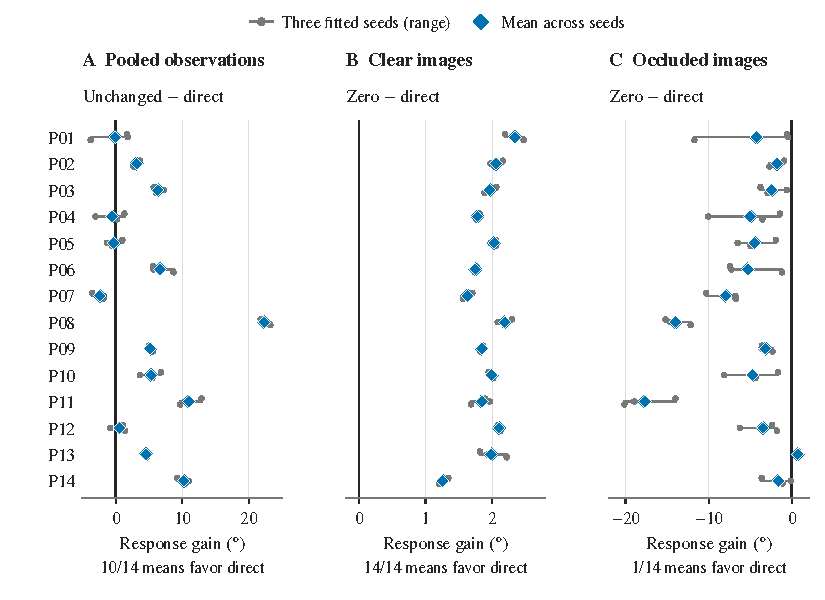
\includegraphics[width=\linewidth]{figures/cases.pdf}
\caption{Participant response profiles, with all 14 development people shown without selection. A: unchanged-minus-direct error, pooled over observations. B--C: zero-minus-direct error for clear and occluded images. Positive values favor jointly fitted direct coordinate restoration. Diamonds average seeds 17, 29, and 43; gray points and horizontal ranges show those fitted values, not confidence intervals. The original 720$\dg$ failure cost and hierarchical aggregation are retained; nonheld/held response strata have 2:1 weighting. Estimators, cameras, naming conditions and physical orientations are pooled. P01--P14 refer to the same people in every panel. Axis ranges differ. These exploratory summaries are not reconstructed poses or clinical examples.}
\label{fig:cases}
\end{figure}
